\documentclass[letterpaper, 10pt, conference]{ieeeconf}
\usepackage{times}


\IEEEoverridecommandlockouts
\overrideIEEEmargins


\usepackage{cite}
\usepackage{graphicx}
\usepackage{relsize}
\usepackage{amssymb,amsmath}
\usepackage{algorithm}
\usepackage{color}
\usepackage[noend]{algorithmic}
\usepackage{flushend}
\usepackage[export]{adjustbox}
\renewcommand{\thefootnote}{\fnsymbol{footnote}}

\newcommand{\Acronym}[1]{\ensuremath{{{\texttt{#1}}}}}
\newcommand{\Symbol}[1]{\ensuremath{\mathcal{#1}}}
\newcommand{\Function}[1]{\ensuremath{{ \textsc{#1}}}}
\newcommand{\Constant}[1]{\ensuremath{{\texttt{#1}}}}
\newcommand{\Var}[1]{\ensuremath{{{\textsl{#1}}}}}
\newcommand{\False}{\Constant{false}}
\newcommand{\True}{\Constant{true}}
\newcommand{\Null}{\Constant{null}}
\newcommand{\Name}{\Function{\small{PARCov}}}
\newcommand{\Revision}[1]{\textcolor{red}{#1}}
\newcommand{\R}{\ensuremath{\mathbb{R}}}
\newcommand{\Traj}{\ensuremath{\zeta}}
\newcommand{\Tree}{\Symbol{T}}
\newcommand{\pair}[1]{\ensuremath{\langle#1\rangle}}

\newcommand{\mychange}[1]{\textcolor{red}{#1}}

\newcommand{\comment}[1]{\textcolor{blue}{#1}}

\newcommand{\argmax}[1]{\underset{#1}{\operatorname{arg}\,\operatorname{max}}\;}
\newcommand{\Max}[1]{\underset{#1}{\operatorname{max}}\;}
\newcommand{\grad}[1]{\underset{#1}{\operatorname{\Function{GradientDescent}}}\;}
\newcommand{\s}{\textbf{s}}

\newcommand{\fig}[1]{Fig~\ref{fig:#1}}

%\setlength{\abovedisplayskip}{1pt}
%\setlength{\belowdisplayskip}{1pt}

\begin{document}

\title{A Planner for Autonomous Risk-Sensitive Coverage
  (\textsc{PARCov}) by a\\
Team of Unmanned Aerial Vehicles}

%\title{A Planner for Autonomous Risk-Sensitive Aerial Coverage ($\textsc{PARACov}$) }

\author{Alex Wallar \and Erion Plaku \and Donald A. Sofge
\thanks{A. Wallar is with the School of Computer Science,
  University of St Andrews, Fife KY16 9AJ, Scotland, UK. E. Plaku is with the
  Dept. of Electrical Engineering and Computer Science, Catholic
  University of America, Washington DC 20064 USA. D. A. Sofge is with
  the Naval Research Laboratory, Washington, DC 20375 USA.
}}


\maketitle
\begin{abstract}

This paper proposes a path-planning approach to enable a team of
unmanned aerial vehicles (UAVs) to efficiently conduct surveillance of
sensitive areas. The proposed approach, termed $\Name$ (Planner for
Autonomous Risk-sensitive Coverage), seeks to maximize the area covered by the
sensors mounted on each UAV while maintaining high sensor data quality
and minimizing detection risk.  $\Name$ uses a dynamic grid to keep
track of the parts of the space that have been surveyed and the times
that they were last surveyed. This information is then used to move
the UAVs toward areas that have not been covered in a long time.
Moreover, a nonlinear optimization formulation is used to determine
the altitude at which each UAV flies. The efficiency and scalability
of $\Name$ is demonstrated in simulation using complex environments
and an increasing number of UAVs to conduct risk-sensitive
surveillance.

\end{abstract}


\section{Introduction}
\label{sec:Intro}

%  why are UAVs important?

%  what problem are we studying?

%  why is that problem important?

%  what have other people done solving similar problems?

%  what new things do we bring?

%  does it open up directions for new research?

UAVs are seen as providing a viable way to enhance automation in
environmental monitoring, search-and-rescue missions, package
delivery, target tracking, and many other applications.  UAVs, such as
ARDrone and AscTec Pelican quadcopters, are becoming more commercially
available, making them also an economically-feasible option for
deployment in autonomous aerial missions.

Towards increasing the autonomy of UAVs, this paper describes an
algorithm for persistent area coverage using multiple cooperative
quadcopters while accounting for the risk and sensor data quality
involved in the coverage. The proposed approach, $\Name$, seeks to
move the quadcopters to promote informed coverage and adjusts the
altitude to maximize sensor data quality while minimizing the
associated risk. Risk plays an important role in many autonomous
aerial missions, especially when seeking to reduce the likelihood of
being detected by a possibly hostile agent. Although this paper
focuses on detection risk, $\Name$ is general and can minimize other
risk metrics that decrease in value as the altitude increases.  For
instance, risk can also be used to model a brushfire. In such
scenario, $\Name$ can provide risk-sensitive aerial
coverage of a wildfire while maximizing the sensor data quality.



%There also
%been active research for 3D path planning for information collection
%using autonomous underwater vehicles~\cite{Yilmaz08,Hover09}.


%UAVs~\cite{Kuhlman14,ErgezerL14,Sydney14,Apker14,Huynh}

There is a burgeoning body of work focusing on aerial missions using
one or several UAVs \cite{ryan2004overview,goerzen2010survey}. Ergezer
and Leblebicio{\u{g}}lu \cite{ErgezerL14} describe an algorithm for 3D
path planning using UAVs that seeks to avoid forbidden regions and
maximize information collection from desired regions.  Nikolos et al.
\cite{nikolos2003evolutionary} develop evolutionary algorithms for
offline/online path planning for UAVs. Kuhlman et al.~\cite{Kuhlman14}
provide an algorithm that optimizes a closed-loop trajectory path for
persistent area coverage by a single UAV that maximizes the
information gained from information-rich areas.  Beard and McLain
\cite{beard2003multiple} take into account communication-range
constraints in order to ensure that UAVs always remain in
communication range as they visit desired regions and avoid forbidden
regions.  Cheng, Keller, and Kumar \cite{cheng2008time} derive a
control policy that generates time-optimal UAV trajectories for urban
structure coverage. Chandler, Pachter, and Rasmussen
\cite{chandler2001uav} propose cooperative control techniques
in order to minimize team exposure to radar
detection. Distributed-task allocation procedures are developed in
\cite{maza2007multiple,jin2003cooperative,lemaire2004distributed} in
order to enhance cooperative searching. Sydney, Paley, and Sofge
\cite{Sydney14} provide a physicomimetic method for target detection
using a group of UAVs. This approach continuously searches the area by
following the gradient of an information surface to track targets
using mutual information between the UAVs. A bio-inspired approach is
proposed in \cite{Apker14} which seeks to model the information of a
search space as a field for grazing and the UAVs as grazing animals
that seek to eat the available information.  This approach has shown
to converge more quickly to total information collection than
traditional lawnmower methods.  Genetic algorithms are used in
\cite{gaudiano2005evolving} to design evolving behaviors that could
increase the autonomy of a swarm of UAVs in carrying out
search-and-destroy missions. Huynh, Enright, and Frazzoli \cite{Huynh}
analyze the persistent-patrol problem for a team of UAVs and propose
several policies to minimize the expected waiting time between the
occurrence and detection time of an incident.



\begin{figure}
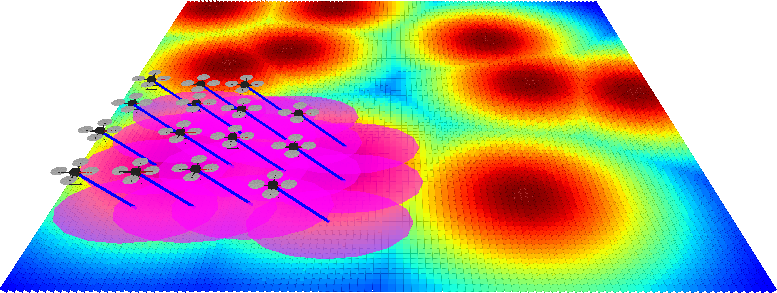
\includegraphics[width=0.49\columnwidth]{usef/rover1.png}
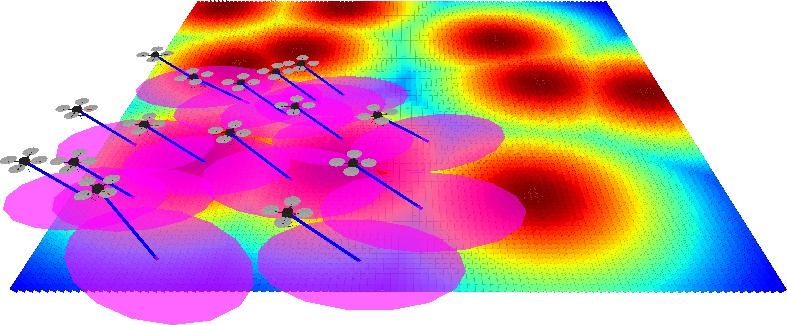
\includegraphics[width=0.49\columnwidth]{usef/rover2.png}\\
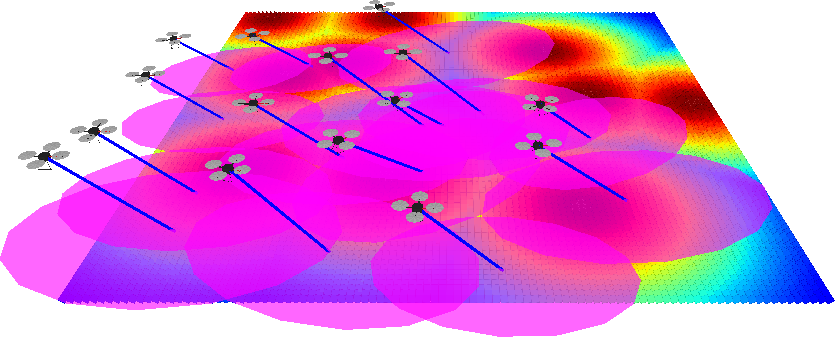
\includegraphics[width=0.49\columnwidth]{usef/rover3.png}
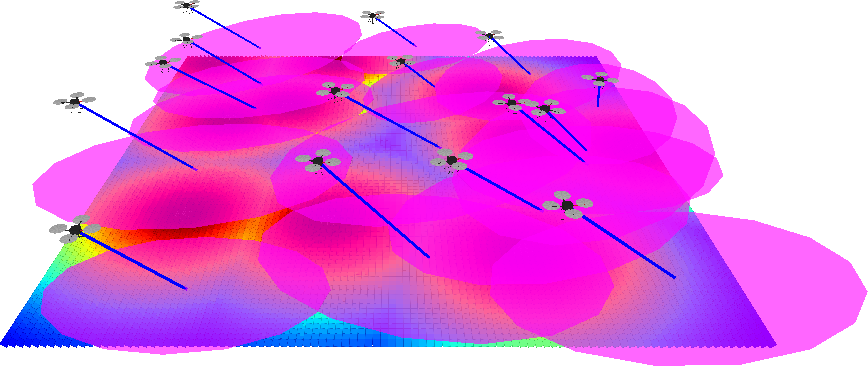
\includegraphics[width=0.49\columnwidth]{usef/rover4.png}
\caption{Snapshots of $\Name$ at different iterations showing how the
  quadcopters cover the designated area. The risk model is shown as a heatmap with red indicating high risk and blue indicating low risk. Figures better viewed in color and on screen.}
\label{fig:cover}
\end{figure}


The proposed approach, $\Name$, offers several contributions. In
particular, it utilizes simple interactions between UAVs to promote an
emergent behavior that maximizes coverage and sensor data quality
while minimizing the risk.  $\Name$ achieves scalability by separating
planning of motions to maximize coverage with adjustments in altitude
to account for sensor data quality and risk. $\Name$ does not try to
avoid forbidden regions, but seeks to mitigate the potential risk. The
efficiency and scalability of $\Name$ is demonstrated in 3D simulation
using complex environments and an increasing number of UAVs to conduct
surveillance.


\section{Problem Formulation}
\label{sec:Problem}
In the problem setting considered in this paper, a number of
quadcopters  are required to survey a given area. The
coverage criteria and the models for sensor data quality and
detection risk are described below.

\paragraph{Area coverage and persistency}
\label{sec:Coverage}  Each quadcopter is
equipped with a sensor which is mounted at a fixed angle $\phi$.  The
team of quadcopters seeks to maximize the area coverage on the
$xy$-plane, where a point is considered covered if it is sensed by at
least one of the quadcopters. More specifically,
the area covered by the quadcopters at time $t$ is given by
$$
\Var{SensedArea}_{q_1}(t) \cup \ldots \cup \Var{SensedArea}_{q_n}(t),
$$ where $n$ denotes the number of quadcopters and
$\Var{SensedArea}_{q_i}(t)$ denotes the area on the $xy$-plane sensed
by the $i$-th quadcopter at time $t$.  The experiments
in this paper consider spotlight sensors, so the sensed area
corresponds to an ellipse, which is a function of the
position and orientation of the quadcopter, the angle $\phi$ at which
the sensor is mounted, and the conic aperture $\alpha$.
Fig.~\ref{fig:cover} provides an illustration of the area covered by
the quadcopters.

As the team of quadcopters may not be sufficiently large to achieve
complete area coverage, another objective of $\Name$ is
to ensure that no part of the space goes too long without being
surveyed. In this way, the quadcopters will not remain still but fly
from one part to the next to ensure that the entire area is
persistently surveyed.

\paragraph{Quality of sensor data}
\label{sec:SQ} A second objective is to maintain high sensor data quality, which is needed
in many applications in order to detect objects of interest in the
area being surveyed.  To model the quality of the sensor data, it is
assumed first that there is an optimal altitude, denoted by
$\mu_\Var{sq}$, to fly the quadcopter in order to achieve the highest
sensor data quality. This optimal altitude depends on the object being
tracked and varies from situation to situation. For example, the
optimal altitude to track a person is much less than the optimal altitude
to track a tank since the tank is larger and moves faster.  In this
paper, the optimal altitude $\mu_\Var{sq}$ is passed to $\Name$ as an
argument by the user.

Furthermore, the sensor data quality is assumed to decrease exponentially
as the deviation from the optimal altitude increases. More precisely,
the sensor data quality is modeled as a distribution with mean
$\mu_\Var{sq}$ and standard deviation $\sigma_\Var{sq}$, i.e.,
$$ SQ(z) = \exp{(-{(\frac{z}{ \cos{\phi}} -
\mu_{sq})^2}/{(2\sigma_{sq}^2)})},
$$
where $z$ is the altitude at which the quadcopter is flying and $\phi$
is the angle at which the sensor is mounted.

\paragraph{Detection risk}
\label{sec:Risk}


While surveying the area, the quadcopters also seek to reduce the risk
of being detected, where a function $R : \R^3 \rightarrow (0, 1)$ determines the
detection risk $R(x, y, z)$ at each location $(x, y, z)$.
In this paper, $R(x, y, z)$ is modeled based on a ground-level risk,
$R_0 : \R^2 \rightarrow (0, 1)$, where $R_0(x, y)$ indicates the risk
of the quadcopter being detected at location $(x, y)$ on the ground
level. More specifically, the ground-level risk is used to scale $R$
as altitude increases with an exponential decay, defined as follows:
$$
 R(x, y, z) = R_0(x, y) \cdot \exp{\left(-\frac{z^2}{K \cdot R_0(x, y)^2}\right)},
$$
where $K$ is a scaling constant. In this way, when the ground-level risk is
high, which would indicate a hostile environment, the quadcopters
would need to fly at high altitudes in order to reduce the
detection risk. When the ground-level risk is low, the quadcopters can
fly at lower altitudes without risking detection.

The ground-level risk $R_0(x, y)$ is modeled by centering normal
distributions around risk points that are given a priori. More
precisely, a set of risk points $\Var{RiskPoints} = \{p_1, \ldots,
p_m\}$ is sampled uniformly at random inside the boundaries of the
area to be surveyed. Each risk point $p_i$ defines a threat that
decreases exponentially as the distance from $p_i$ increases. Then,
$R_0(x, y)$ is defined as
$$ R_0(x, y) = \Max{p \in \Var{RiskPoints}}
\exp{\left(-\frac{||p - (x, y)||_2}{L}\right)},
$$
where $L$ is a scaling constant.
An illustration of $R_0(x, y)$ is provided in Fig.~\ref{fig:Heatmap}.
\begin{figure}[h]
\centering
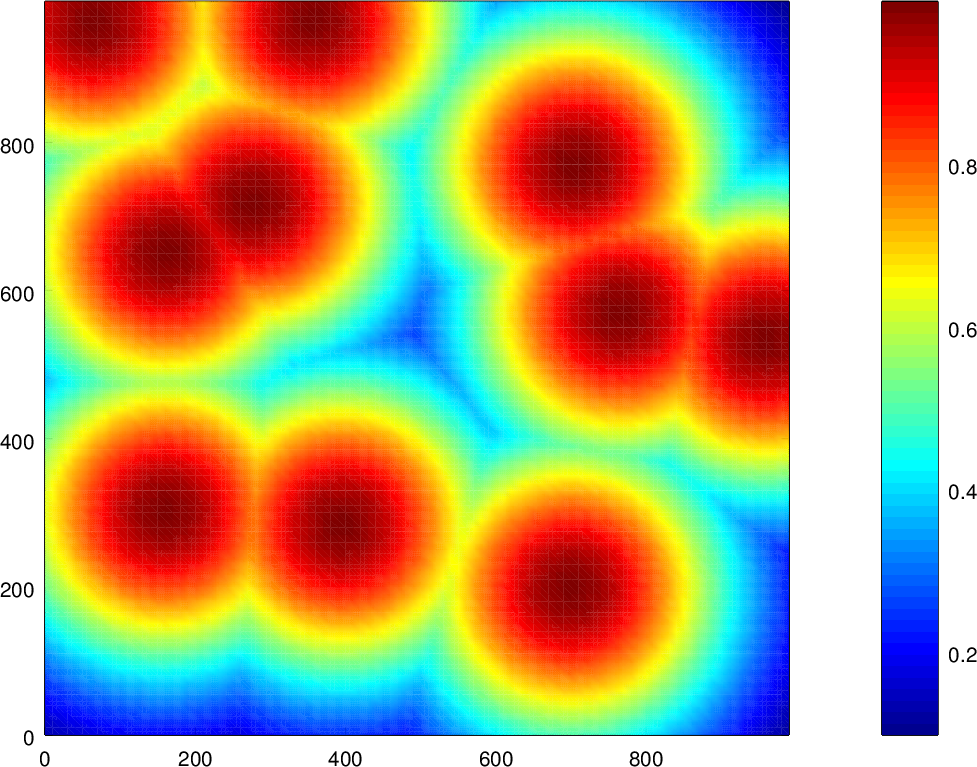
\includegraphics[width=0.8\columnwidth]{usef/heatmap.png}
\caption{Illustration of the ground-level risk $R_0(x, y)$
  corresponding to the case of $10$ randomly-sampled risk
  points. Color intensity indicates risk values.}
\label{fig:Heatmap}
\end{figure}
\paragraph{Problem statement}
\label{sec:ProblemStatement}
Putting it all together, the problem considered in this paper can be
stated as follows: Given an area to be surveyed, models for sensor data
quality and detection risk, and an initial placement of the
quadcopters, move the quadcopters so that they maximize area
coverage, ensure that no part of the space goes too long without being
surveyed, maintain high sensor data quality, and reduce the detection risk.

\section{Method}
\label{sec:Method}

To achieve the stated objectives, $\Name$ splits planning into two
stages: (i) planning the quadcopters' motions in $xy$ to promote area
coverage and persistency and (ii) planning for the altitude
to minimize the detection risk and maximize sensor data quality. Pseudocode
is provided in Alg.~\ref{algo:planning}. Descriptions of the main
steps of the algorithm follow.


\begin{algorithm}[ht]

\caption{Pseudocode for $\Name$}

\label{algo:planning}


\begin{algorithmic}[1]


\setcounter{ALC@line}{0}

\vspace*{1mm}

\STATE $\Symbol{G} \leftarrow \Function{InitGrid()}$

\WHILE{$\Function{finished()} = \False$}

\FOR{$q \in \Var{Quadcopters}$}
\STATE $(v', \beta') \leftarrow
\Function{GetDirectionAndOrientation}(q,\Symbol{G})$


\STATE $\begin{bmatrix}
    x' \\[0.2em]
    y'
\end{bmatrix} \leftarrow \begin{bmatrix}
    q.x \\[0.2em]
    q.y
\end{bmatrix} + \Var{step} \cdot \mathlarger{\frac{v'}{||v'||}}$
\STATE $z' \leftarrow \Function{DetermineAltitude}(x', y')$
\STATE $\Function{SetPositionAndOrientation}(q, x', y', z', \beta')$
\STATE $\Function{UpdateGrid}(\Symbol{G}, q)$

\ENDFOR

\ENDWHILE

\end{algorithmic}
\end{algorithm}

\subsection{Planning to promote area coverage and persistency}
\label{sec:Planning2D}

First, $\Name$ imposes a grid over the $xy$ bounding box of the area
being surveyed. The grid, denoted by $\Symbol{G}$, is used to keep
track of the parts of the space that have been surveyed and the times
that they were last surveyed (Alg.~\ref{algo:planning}:1). Whenever a
grid cell $c$ is sensed by some quadcopter, i.e., $c \in
\Var{SensedArea}_{q_i}(t)$,  the current time $t$ is stored in that grid cell
(Alg.~\ref{algo:planning}:8).
An illustration of the grid $\Symbol{G}$ at some
time instance is provided in
Fig.~\ref{fig:timegrid}.

\begin{figure}[h]
\centering
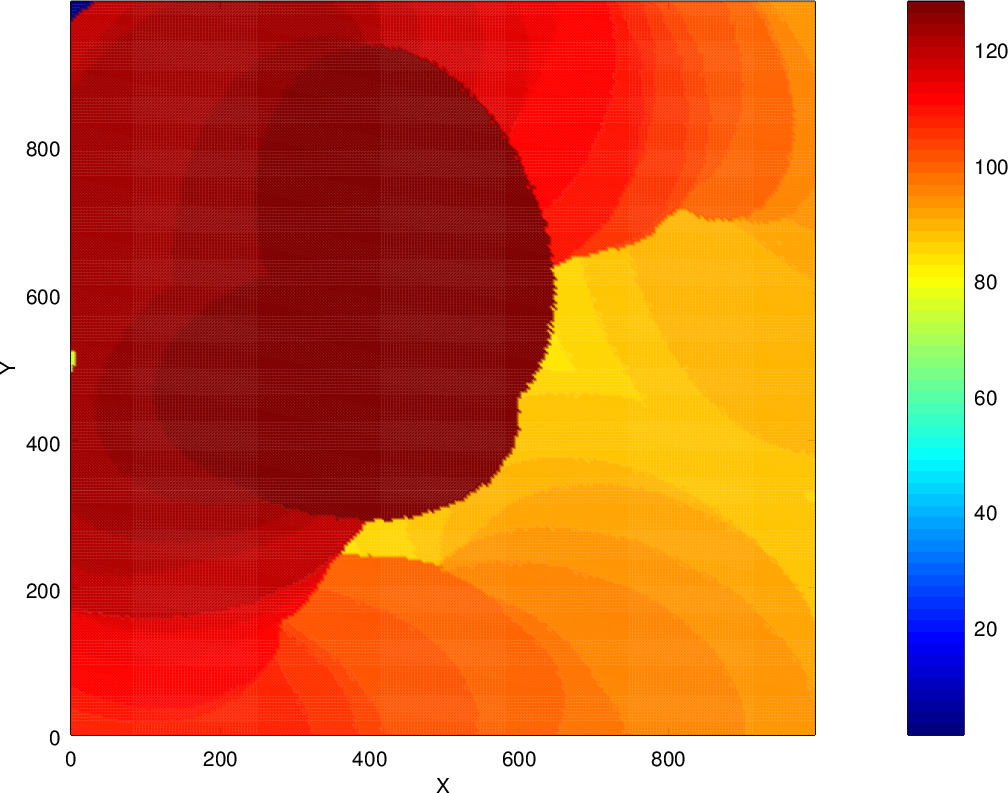
\includegraphics[width=0.7\columnwidth]{usef/grid}

\caption{An instance of the grid $\Symbol{G}$ where the color in the spectrum
denotes the time (as iteration count) that the cell at $x, y$ was visited, i.e., red denotes recently-visited areas.}
\label{fig:timegrid}
\end{figure}

\noindent
$\Name$ uses the grid $\Symbol{G}$ to determine the new direction
and orientation of each
quadcopter. Pseudocode is given in Alg.~\ref{algo:2dplanning}. In
particular, $\Name$ seeks to move a quadcopter $q$ toward areas that
have not been covered in a long time. In order to take advantage of
locality, $\Name$ considers the vicinity of the area sensed by $q$
at the current time.

To determine the new direction and new orientation, $\Name$ first uses
random sampling to generate a set of candidate orientations
(Alg.~\ref{algo:2dplanning}:2). Let $\Var{SensedArea}(\beta)$ denote
the area that would be sensed by $q$ when setting its orientation to
$\beta$ (keeping the position fixed). As an example, for the spotlight
sensor model used in the experiments, the sensed area would be an
ellipse defined parameterically with respect to $\omega \in [0, 2\pi]$ as follows:
$$
\begin{bmatrix}
x\\
y
\end{bmatrix} +
\Var{Rot}(\beta) \cdot \begin{bmatrix} z \cdot
    \tan({\phi} - \alpha) +
    A_M \cdot (1 + \cos{\omega})  \\[0.2em]
    A_m \cdot
\sin{\omega} \end{bmatrix},
$$
where $(x, y, z)$ is the position of the quadcopter, $\Var{Rot}(\beta)$ is the 2D-rotation matrix,
$ A_M = z \cdot \tan{(\phi + \alpha)} - z \cdot
\tan{\phi}$ is the major axis, and $A_m = \frac{z \cdot
  \tan{\alpha}}{\cos{\phi}} $ is the minor axis.


Next, $\Name$ generates a number of segments along $\xi(\beta)$, where
$\xi(\beta)$ denotes $\Var{SensedArea}(\beta)$ enlarged by some
$\epsilon > 0$ (Alg.~\ref{algo:2dplanning}:4--5). The $i$-th segment
is generated by connecting the points on the perimeter of $\xi(\beta)$
corresponding to the angles $(i-1)\zeta$ and $(i+1) \zeta$, where
$\zeta$ is a user-defined parameter (set to $10^{\circ}$).  The
average wait time for a segment $s$, denoted by
$\Var{AvgWaitTime}(\Symbol{G}, s)$, is computed by considering a
number of equally-spaced points along the segment $s$, where
$\Var{WaitTime}(\Symbol{G}, x, y)$ denotes the number of iterations
that have passed since the point $(x, y)$ was last sensed by some
quadcopter.  Note that this information is obtained from the grid
$\Symbol{G}$ by looking up the iteration number associated with the
grid cell that contains $(x, y)$ and subtracting the value of the grid
cell from the current iteration number.

The quadcopter $q$ will move toward the segment $s$ with the maximum
average wait time, i.e.,
$$
s = \argmax{s' \in \Var{AllSegments}} \Var{AvgWaitTime}(\Symbol{G}, s')
$$
where
$
\Var{AllSegments} = \bigcup_{\beta \in \Var{orientations}} \Var{segments}(\xi(\beta)).
$

\noindent
The new orientation of the quadcopter $q$ is set to the candidate
orientation $\beta$ from which the $\xi(\beta)$ that contains the segment
$s$ was derived (Alg.~\ref{algo:2dplanning}:11). The new direction is
set by taking a weighted average of the equally-spaced points along
the segment $s$ (Alg.~\ref{algo:2dplanning}:12--13), i.e.,
$$
- (q.x, q.y) + \sum_{(x, y) \in \Var{points}(s)}
\frac{\Var{WaitTime}(\Symbol{G}, x, y)}{t} (x, y),
$$
where
$
t = \sum_{(x', y') \in \Var{points}(s)} \Var{WaitTime}(\Symbol{G}, x', y').
$

This rule has desirable emergent properties for the team of
quadcopters.  Since the quadcopters share the same grid $\Symbol{G}$,
they will act cooperatively to fill the unvisited space without having
to explicitly coordinate with one another. In particular, each
quadcopter will move towards an area in its vicinity that has a large
average wait time.  This makes it less likely for the quadcopters to
clutter together. Suppose two or more quadcopters are moving towards
the same segment. When a quadcopter senses the segment, its wait time
becomes zero, which causes the other quadcopters to move towards other
segments. Furthermore, since the segment selected by each quadcopter
$q$ is in the vicinity of the area sensed by $q$, then it
is likely that $q$ will reach it first, hence further reducing the
likelihood of clutter.

Moreover, this planning is not dependent on the
number of quadcopters.  If a quadcopter leaves the area, it would
simply no longer update the grid $\Symbol{G}$. The other quadcopters
would have no knowledge that it left and would still be able to
persistently cover the area being surveyed.
This is particularly important for missions
that combine persistent coverage and target tracking. The
persistent coverage can be used to determine the positions
of targets, and a sub-swarm of quadcopters can be deployed
from the group to track the targets while the rest
continues to provide coverage.


\begin{algorithm}[t]
\caption{$\Function{GetDirectionAndOrientation}(q, \Symbol{G})$}
\label{algo:2dplanning}

\begin{algorithmic}[1]

\setcounter{ALC@line}{0}

\vspace*{1mm}


\STATE $\Var{waitTime} \leftarrow -\infty; v' \leftarrow (0,0);
\beta' \leftarrow 0$


%\STATE $\Var{major} \leftarrow q.z \cdot (\tan{(\phi + \alpha)} - \tan{\phi}) + \epsilon$
%\STATE $\Var{minor} \leftarrow q.z \cdot \frac{\tan{\alpha}}{\cos{\phi}} + \epsilon$

\STATE $\Var{orientations} \leftarrow \Function{GetRandomSamples}(0, 2\pi)$

\FOR{$\beta \in \Var{orientations}$}

\STATE $\xi \leftarrow \Function{EnlargedEllipse}(q.x, q.y,
q.z, \beta, \phi, \alpha, \epsilon)$

\STATE $\Var{segments} \leftarrow \Function{GetSegments}(\xi)$


\FOR{$s \in \Var{segments}$}
\STATE $\Var{points} \leftarrow \Function{GetPoints}(s)$
\STATE $t \leftarrow \sum_{(x, y) \in \Var{points}}
\Var{WaitTime}(\Symbol{G}, x, y)$

%\STATE $x \leftarrow q.z \cdot \tan{(\phi - \alpha)} + \Var{major} \cdot (1 + \cos{\omega})$
%\STATE $y \leftarrow \Var{minor} \cdot \sin{\omega}$

%\STATE $\begin{bmatrix}
%    \hat{x} \\[0.2em]
%    \hat{y}
%\end{bmatrix} \leftarrow \begin{bmatrix}
%    \cos{\beta} & -\sin{\beta} \\[0.2em]
%    \sin{\beta} & \cos{\beta}
%\end{bmatrix} \cdot \begin{bmatrix}
%    x \\[0.2em]
%    y
%\end{bmatrix} + \begin{bmatrix}
%    q.x \\[0.2em]
%    q.y


\IF{$\Var{waitTime} < t / |\Var{points}|$}
\STATE $\Var{waitTime} \leftarrow t / |\Var{points}|$
\STATE $\beta' \leftarrow \beta$
\STATE
$(\bar{x}, \bar{y}) \leftarrow \sum_{(x, y) \in \Var{points}}
 \frac{\Var{WaitTime}(\Symbol{G}, x, y)}{t} \cdot (x, y)$

\STATE $v' \leftarrow (\bar{x} - q.x, \bar{y} - q.y)$
\ENDIF
\ENDFOR
\RETURN $(v', \beta')$


\ENDFOR %orientations
\end{algorithmic}
\end{algorithm}


\subsection{Determining the altitude}
\label{sec:Altitude}
To determine the altitude, $\Name$ optimizes an objective function
that maximizes the sensor data quality and
minimizes the detection risk, i.e.,
$$
J(x, y, z) = SQ(z) - R(x, y, z).
$$
Therefore, the optimal altitude can be determined by finding the $z$ value
that maximizes $J$ for a given $x, y$, i.e.,
$$ \Function{DetermineAltitude}(x, y) = \argmax{z \in [z_{min}, z_{max}]} J(x, y,
z).
$$
Nonlinear optimization solvers can then be used to numerically compute
the optimal altitude (this paper uses SciPy, which is open source).

After determining the altitude, the quadcopter is set at the new
position and orientation (Alg.~\ref{algo:planning}:18). The grid is updated accordingly to account
for the new sensed area. Since the grid is
shared among the quadcopters, the change in altitude of one quadcopter
would cause a change in the sensed area,
which could potentially change which parts of the grid are covered. As
a result, the rest of the group will react to this new information. In
particular, if a quadcopter decreases its altitude, then there will be
more uncovered space around it so the rest of the quadcopters will
move to cover this space. These dynamic adjustments, as shown by the
experimental results, make it possible to efficiently and persistently
cover the area being surveyed while maintaining high sensor data quality
and reducing the detection risk.




\section{Experiments and Results}
\label{sec:ExpResults}

Experiments are conducted in simulation with an increasing number of
quadcopters and risk points.

\subsection{Experimental Setup}
\subsubsection{Scenes}
A scene is defined by its dimensions and the number and location of
the risk points. Three scene dimensions were used: small ($600 \times
600 \times 160$), medium ($1000 \times 1000 \times 160$), and large
($2000 \times 2000 \times 160$). The risk points were randomly placed
inside the $xy$ bounding box. The generated scenes are referred to as
$\Var{sceneX}\_n$, where $\Var{X} \in \{\Var{small}, \Var{medium},
\Var{large}\}$, and $n \in \{1, 3, 5, \ldots, 21\}$.  The quadcopters
all started in a square formation at the top left of the scene.  The
number of quadcopters was varied as $1, 6, 11, 16, 21, 26$.

\subsubsection{Performance criteria}
\label{sec:Performance}
Results report on the average percentage of the total area coverage,
the average sensor data quality, the average risk, and average wait
time in the grid $\Symbol{G}$. The sensor data quality and risk
metrics were determined using the same functions as in the
optimization process (Section~\ref{sec:Problem}).

Area coverage was computed using a Monte-Carlo process where a large
number of random points (1000) were sampled inside the $xy$ bounding
box of the scene. At each iteration of $\Name$, each sampled point is
checked whether or not it is sensed by some quadcopter. The ratio of
the number of sampled points which are within any of the sensed areas
to the total number of sampled points was used to determine the
percentage of the total area covered.

The average wait time is used to show that no part of the area being
surveyed goes for too long a time without being sensed.  This metric
was computed at each iteration as
$$\frac{1}{|\Var{cells}(\Symbol{G})|}\sum_{c \in
  \Var{cells}(\Symbol{G})} \Var{WaitTime}(\Symbol{G}, c).$$
Recall that $\Var{WaitTime}(\Symbol{G}, c)$ corresponds to the number
of iterations since the last time $c$ was sensed by some quadcopter.

\subsubsection{Hardware and software}  Experiments are conducted on an Intel
Core i7 machine (CPU: 2.40GHz, RAM: 16GB) using Ubuntu 14.04. Code
was written in Python 2.7.  ROS rviz was used for visualization.

\subsection{Results}

Before presenting quantitative results, we provide some qualitative
illustrations to show $\Name$ in action.  Fig.~\ref{fig:cover} shows
how the quadcopters cover the designated area. Using the information
from the grid $\Symbol{G}$, the quadcopters start moving toward the
uncovered areas.


\begin{figure}[t]
\centering
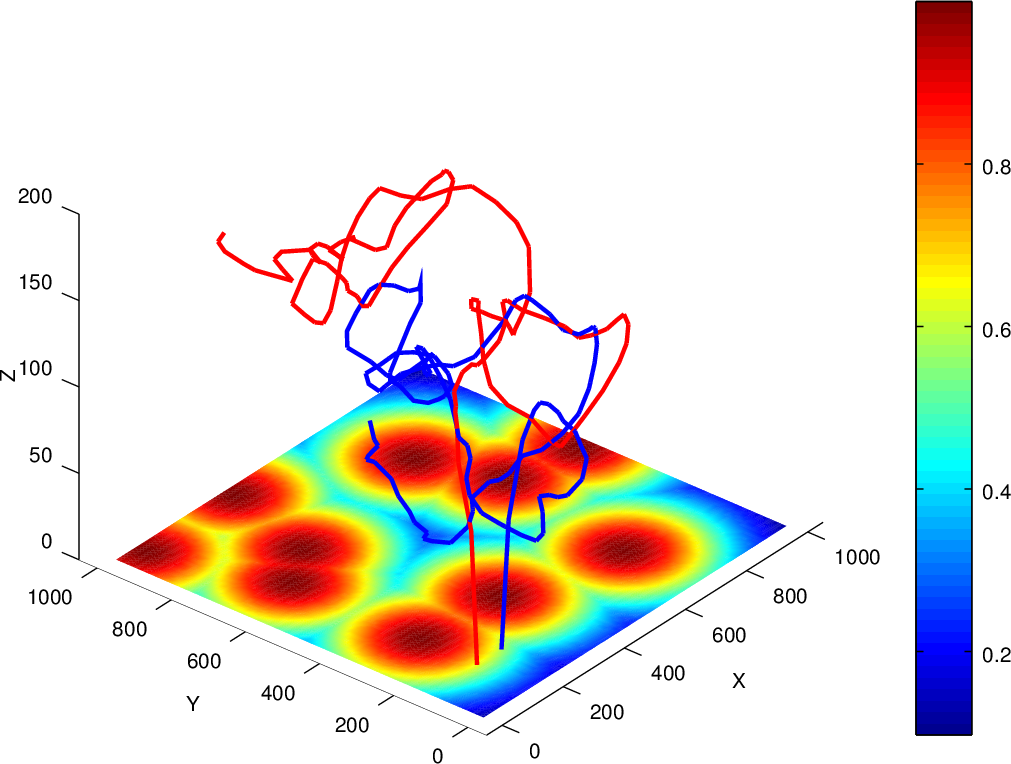
\includegraphics[width=0.8\columnwidth]{usef/trajectories}

\caption{Trajectories taken by two quadcopters shown in blue and red,
respectively. The initial risk $R_0$ is shown as a heatmap (a different color scheme is used here to better visualize the trajectories). }

\label{fig:Trajs}
\end{figure}

Another illustration of $\Name$ in action is provided in
Fig.~\ref{fig:Trajs}, which shows  trajectories
taken by two quadcopters. Note how the quadcopters increase their
altitude when surveying areas designated as high risk and reduce their
altitude when going over low-risk areas. As discussed in
Section~\ref{sec:Altitude}, $\Name$ uses a nonlinear optimization
process to reduce detection risk while maintaining
high sensor data quality.


\subsubsection{Performance as a function of the number of iterations}
Fig.~\ref{fig:ResTimeline}
shows that in a small number of iterations, regardless
of the number quadcopters or number of risk points, the team of quadcopters
was able to achieve high coverage of the designated
area. In fact, at around 20 iterations the coverage was over 90\%
for each of the scenarios. An iteration corresponds to computing one
move (position and orientation) for each quadcopter
(Alg.~\ref{algo:planning}:4--8). As shown in
Fig.~\ref{table:TimeIter}, $\Name$ scales linearly with the number of
quadcopters.

%\begin{table}
%\centering
%{\small{
%\begin{tabular}{r|cccccc}
%nr. quadcopters & 1 & 6 & 11 & 16 & 21 & 26\\\hline
%mean [s] & 0.03 & 0.20 & 0.35 & 0.48 & 0.61 & 0.73\\
%std & 0.01 & 0.02 & 0.04 & 0.06 & 0.06 & 0.09\\
%\end{tabular}
%}}

\begin{figure}
\centering
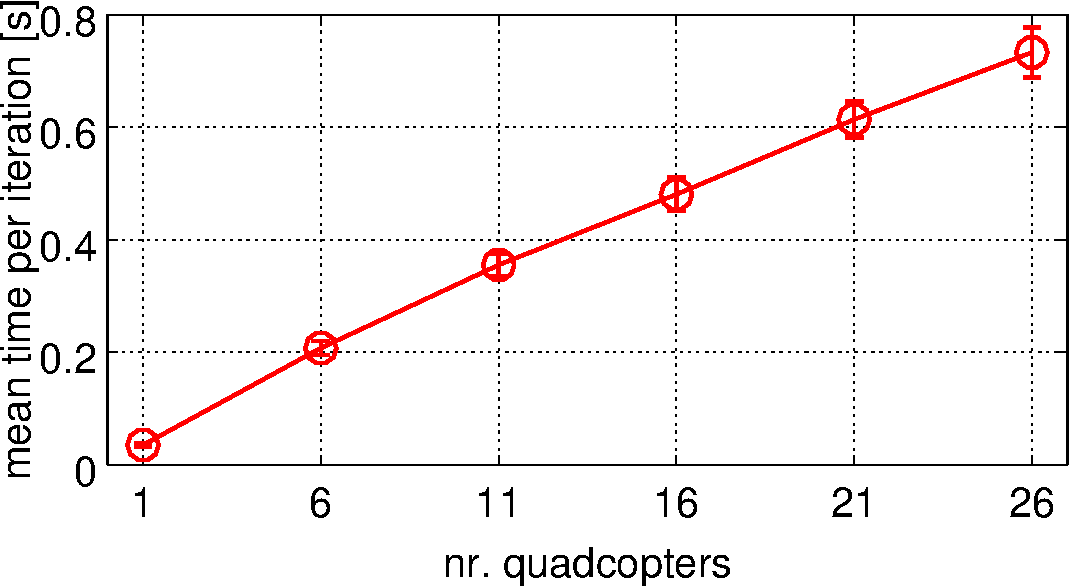
\includegraphics[width=0.8\columnwidth]{figResTimePerIter}
\caption{Runtime per iteration. Bars indicate standard deviation.}
\label{table:TimeIter}
%\end{table}
\end{figure}

Results in Fig.~\ref{fig:ResTimeline} also show that the detection
risk rapidly decreased.  To test the ability of the approach to reduce
the detection risk, in the experiments the quadcopters started at the
minimum viable height, which carries the highest risk. The quadcopters
were quickly able to readjust their height to minimize the risk.
Likewise, the sensor data quality rapidly increased as the iterations
increased because the quadcopters quickly determined the optimal
altitude.  We also notice that the sensor data quality, coverage,
and detection risk did not change much as the number of risk points
increased. This is because the quadcopters are able to spread out
appropriately and reconfigure the altitude in order to maximize the
sensor data quality and minimize the detection risk.

\begin{figure}
\centering
%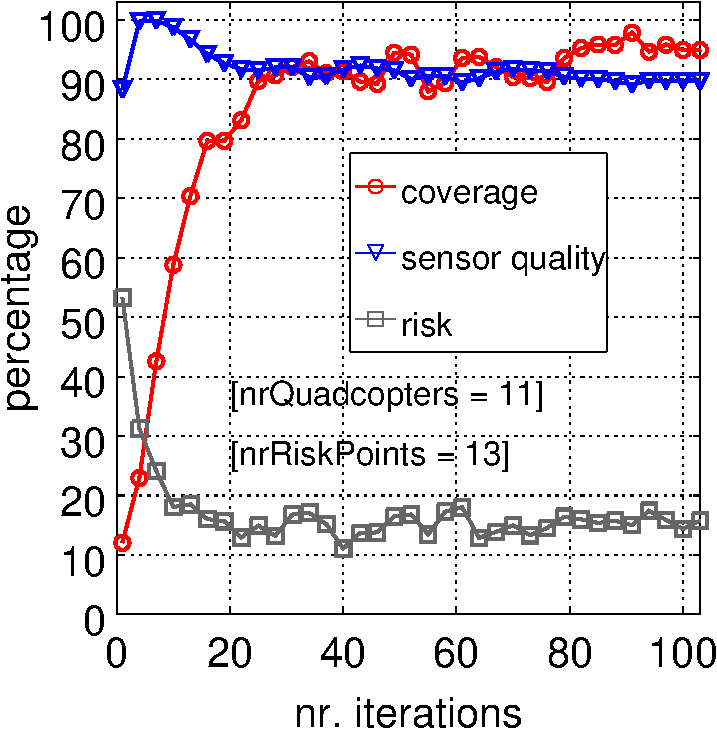
\includegraphics[width=0.3\columnwidth]{figs/figResTimelineR13Q11}
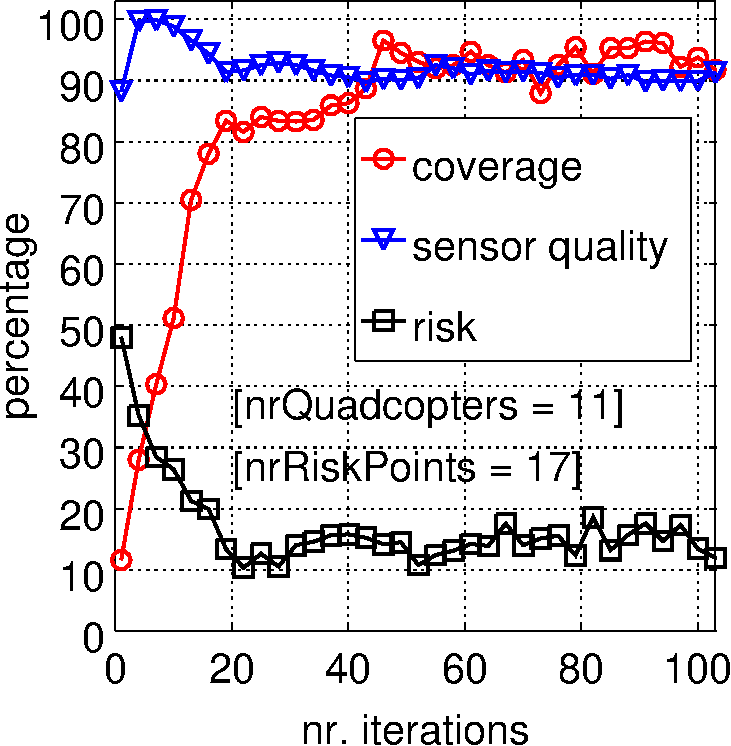
\includegraphics[width=0.48\columnwidth]{usef/figResTimelineR17Q11}
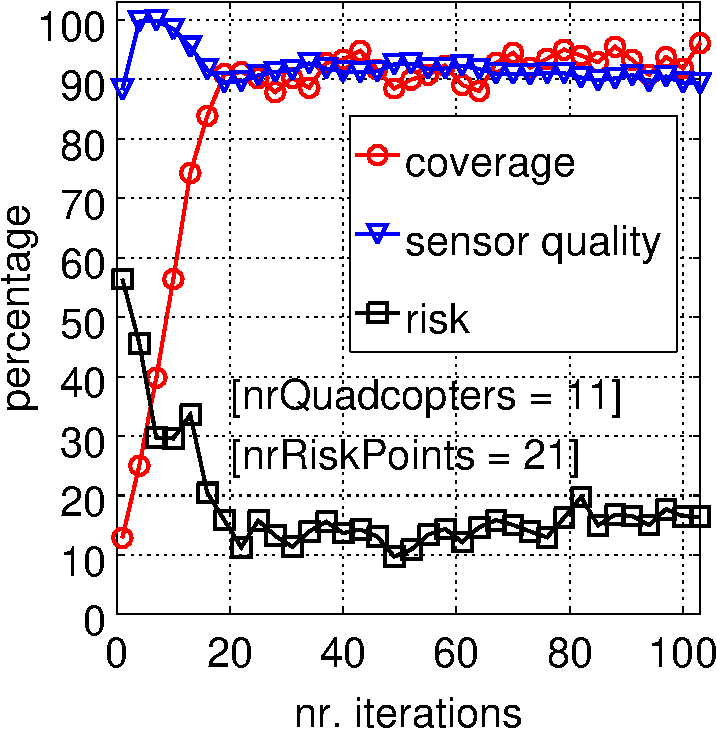
\includegraphics[width=0.48\columnwidth]{usef/figResTimelineR21Q11}\\[2mm]
%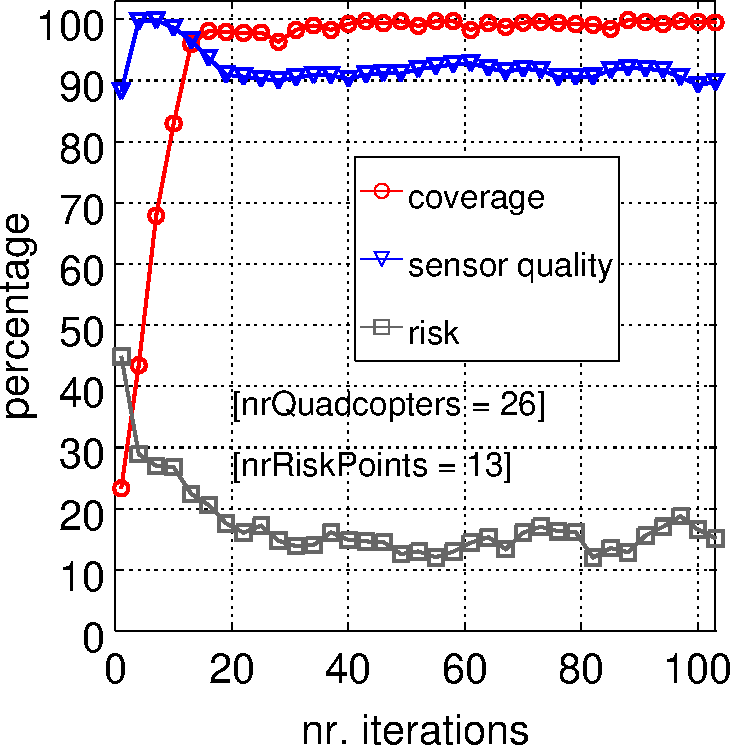
\includegraphics[width=0.3\columnwidth]{figs/figResTimelineR13Q26}
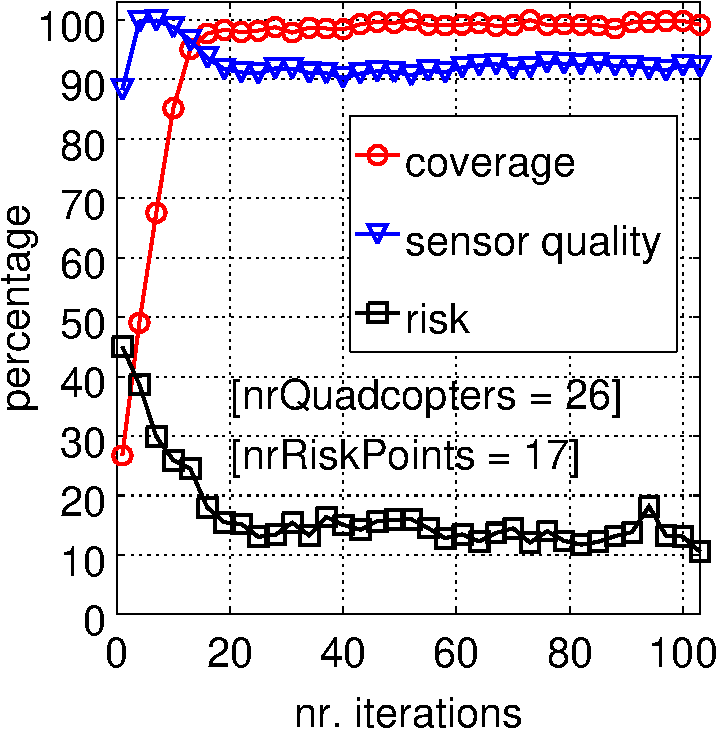
\includegraphics[width=0.48\columnwidth]{usef/figResTimelineR17Q26}
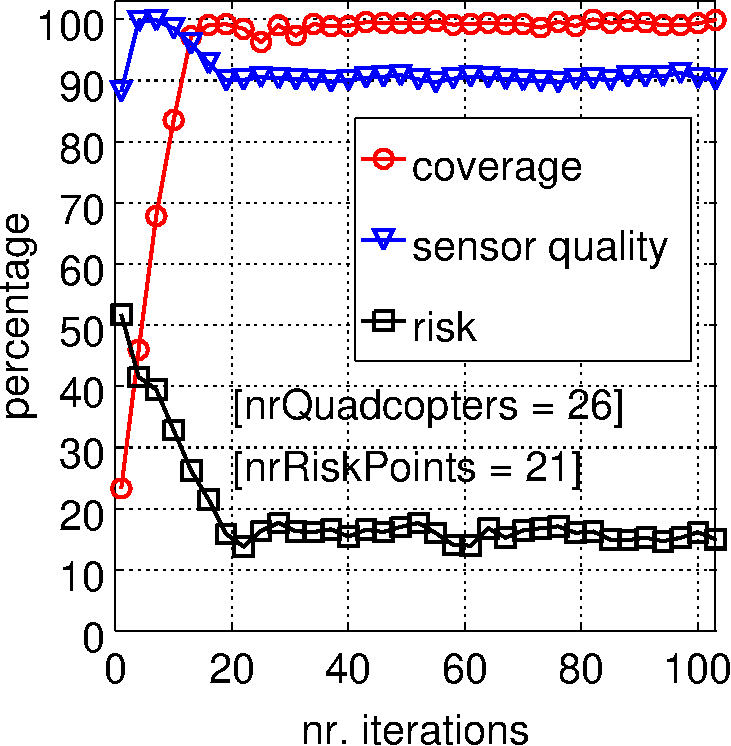
\includegraphics[width=0.48\columnwidth]{usef/figResTimelineR21Q26}
\caption{Performance criteria as a function of the number of
  iterations. Results are shown for instances of the medium-size scene
  with different numbers of risk points and quadcopters.}
\label{fig:ResTimeline}
\end{figure}

\subsubsection{Performance as a function of the number of quadcopters}
Results in Fig.~\ref{fig:ResQuads} show the performance criteria as
the number of quadcopters is increased. As expected, the area coverage
increases as more quadcopters participate in the task. The increase in
coverage is very rapid initially and slows down as the
required number of quadcopters to ensure complete coverage is reached.
These results indicate that $\Name$ effectively dispatches the
quadcopters to fly over uncovered areas. Moreover, $\Name$ keeps the
detection risk low and the sensor quality high even as the number of
quadcopters is increased. The same trends are observed even when
increasing the number of risk points (Fig.~\ref{fig:ResQuads} plots the
performance criteria as a function of the number of quadcopters for three
different scenarios obtained by varying the number of risk points).

\begin{figure*}
\centering
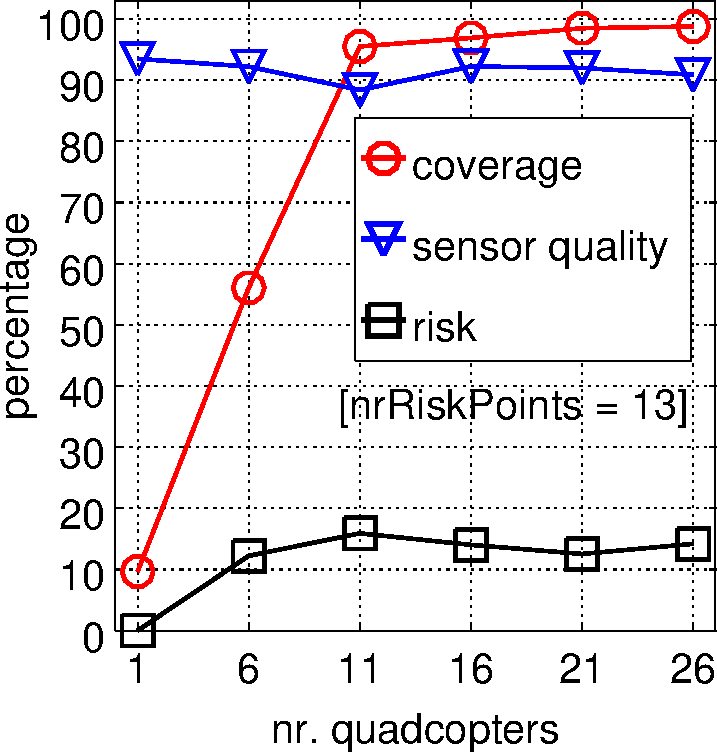
\includegraphics[width=0.28\textwidth]{usef/figResQuadsR13}
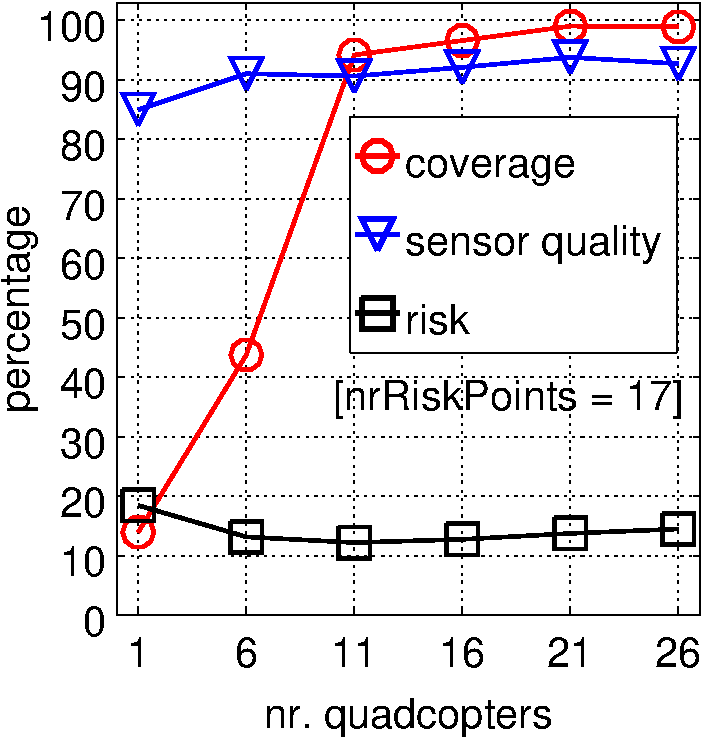
\includegraphics[width=0.28\textwidth]{usef/figResQuadsR17}
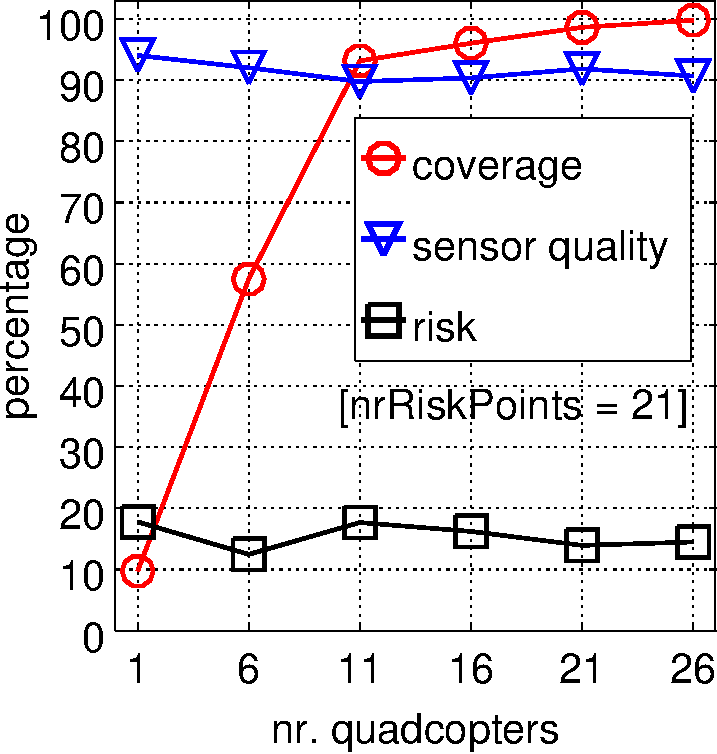
\includegraphics[width=0.28\textwidth]{usef/figResQuadsR21}
\caption{Performance criteria as a function of the number of
  quadcopters. Shown percentages are computed after 250 iterations of
  the algorithm. Results are shown for instances of the medium-size
  scene with different numbers of risk points.}
\label{fig:ResQuads}
\end{figure*}

\subsubsection{Wait times}
Table~\ref{table:ResWaitTimes} shows the average wait time
(Section~\ref{sec:Performance}) as a function of the number of quadcopters.
As the number
of quadcopters increases, the average wait time decreases since
the quadcopters spread through the space
cooperatively and therefore cover the space more quickly.


\begin{table}[h]
\begin{tabular}{r|cccccc}
nr. quadcopters & 1 & 6 & 11 & 16 & 21 & 26 \\\hline
awt [nrRiskPts=13] & 37.90 & 2.19 & 0.14 & 0.08 & 0.03 & 0.03 \\
awt [nrRiskPts=17] & 37.14 & 3.09 & 0.18 & 0.12 & 0.06 & 0.04 \\
awt [nrRiskPts=21] & 35.53 & 1.89 & 0.19 & 0.11 & 0.06 & 0.02
\end{tabular}

\caption{Average wait time (awt).}
\label{table:ResWaitTimes}
\end{table}


\subsubsection{Performance as a function of scene size}
Table~\ref{table:ResScene} shows the performance of $\Name$ on three
different scene sizes: small, medium, and large. In all cases, $\Name$
efficiently covers the area while maintaining high-sensor quality and low detection risk. As expected,
more quadcopters are needed to cover the large scene.

\begin{table}[h]
\begin{tabular}{l|p{3mm}p{3mm}p{3mm}p{3mm}p{3mm}p{3mm}p{3mm}p{3mm}}
nr. quadcopters & 1 & 6 & 11 & 16 & 21 & 26 & 30 & 35 \\\hline
(A) coverage   & 51\% & 95\% & 98\% & 99\% & 99\% & 99\% & 99\% & 99\%\\
(B) coverage & 13\% & 43\% & 94\% & 96\% & 99\% & 99\% & 99\% & 99\% \\
(C) coverage & 3\% & 26\% & 44\% & 54\% & 62\% & 77\% & 84\% & 93\%\\\hline
(A) sensor quality   & 88\% & 92\% & 92\% & 92\% & 91\% & 92\% & 92\%
& 92\%\\
(B) sensor quality & 84\% & 91\% & 90\% & 92\% & 93\% & 92\% & 92\% & 92\%\\
(C) sensor quality & 90\% & 90\% & 89\% & 91\% & 89\% & 90\% & 89\% & 90\% \\\hline
(A) risk   & 27\% & 12\% & 13\% & 14\% & 15\% & 15\% & 15\% & 15\% \\
(B) risk & 18\% & 13\% & 12\% & 12\% & 13\% & 14\% & 14\% & 14\%\\
(C) risk & 15\% & 16\% & 19\% & 14\% & 16\% & 15\% & 16\% & 15\%
\end{tabular}

\caption{(a) small scene: 600x600x200 (b) medium scene: 1000x1000x200 (c) large
scene: 2000x2000x200. In all cases, nrRiskPts=17.}

\label{table:ResScene} \end{table}


\subsubsection{Performance as a function of the projection angle}
Fig.~\ref{fig:ResCamera} provides a summary of the results when
varying the angle $\phi$ at which the sensor is attached to the
quadcopter. As shown, $\Name$ works well for a variety of
values.

\begin{figure}
\centering
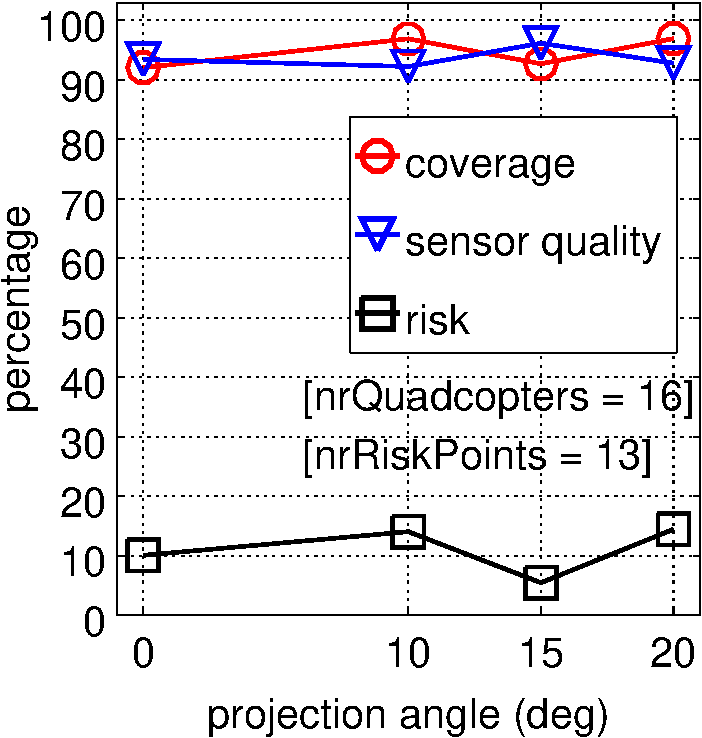
\includegraphics[height=1.3in]{usef/figResCameraR13Q16}
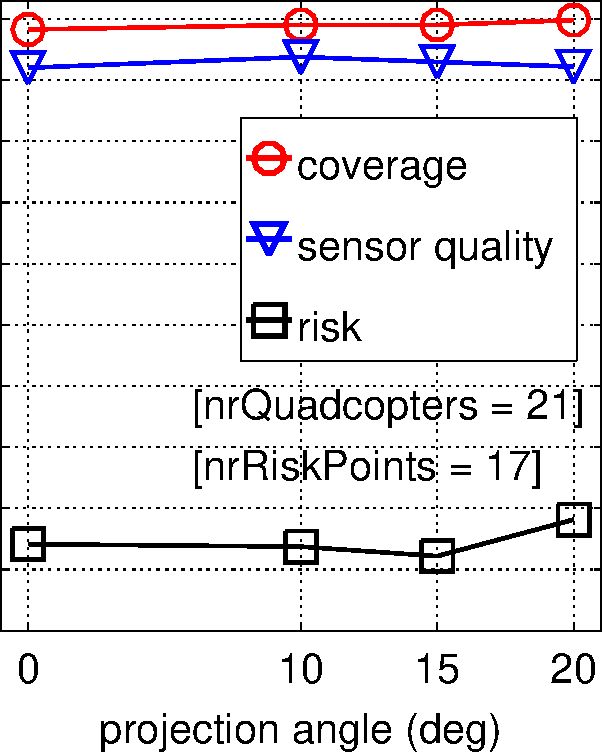
\includegraphics[height=1.3in]{usef/noy/figResCameraR17Q21}
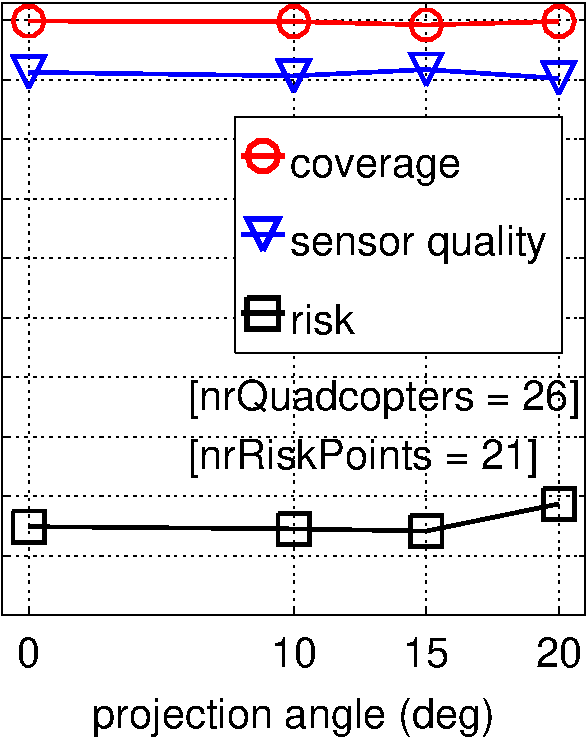
\includegraphics[height=1.3in]{usef/noy/figResCameraR21Q26}
\caption{Performance criteria as function of the angle at which the
  sensor is attached to the quadcopter. Shown percentages
are computed after 250 iterations of the algorithm. Results are
shown for the medium-size scene with different numbers of risk points and
quadcopters.} \label{fig:ResCamera}
\end{figure}



\section{Discussion}

This paper developed a path-planning approach to enable a team of
quadcopters to efficiently conduct surveillance. $\Name$
achieved scalability by separating planning of motions to maximize
coverage with adjustments in altitude to account for sensor data quality
and detection risk.  The efficiency and scalability of $\Name$ was
demonstrated in simulation using complex environments and an
increasing number of UAVs to conduct surveillance.  In future
work, we will enhance the approach to track moving targets. Another
direction for future research is to further improve the sensor quality
by reducing the motion blur. We are also working on using the approach
on a team of ARDrone and AscTec Pelican quadcopters. In order to
execute the planned motions, the approach will be complemented with PD
controllers.

\section*{Acknowledgment}
This work was performed at the Naval Research Laboratory and was
funded by the US Department of Defense, Office of Naval Research under
grant number N0001413WX21045, ``Mobile Autonomous Teams for Navy
Information Surveillance and Search (MANTISS).'' The views, positions
and conclusions expressed herein reflect only the authors’ opinions
and expressly do not reflect those of the US Department of Defense,
Office of Naval Research, or the Naval Research Laboratory.


\bibliographystyle{IEEEtran} \bibliography{mp,plaku,quads}


\end{document}

